\documentclass[11pt]{article}

\usepackage[scaled]{helvet}
\renewcommand\familydefault{\sfdefault} 
\usepackage[T1]{fontenc}
\usepackage{url}
\usepackage[breaklinks]{hyperref}
\def\UrlBreaks{\do\/\do-}
\usepackage{siunitx}
\usepackage{hepnames}
\usepackage{hepparticles}
\usepackage{cite}
\usepackage[utf8]{inputenc}
\usepackage[american]{babel}
\usepackage{graphicx}
\usepackage{subcaption}
\usepackage{tikz}
\usepackage{soul}

  
% shortcut for location of graphics file
\graphicspath{ {./fig/} }

\usepackage{cite}
\usepackage[top=1in, bottom=1in, left=1in, right=1in, paperwidth=8.5in, paperheight=11in]{geometry}

% some hard-coded definitions for some math symbols to be used more easily
\def \et {E_{T}}
\def \met {\not\!\!\et }
\def \alqed {\alpha_{\mathrm{em}}}
\def \GF {G_{\mathrm{F}}}
\def \mtop {M_{\mathrm{t}}}
\def \mH {M_{\mathrm{H}}}
\def \mX {M_{\mathrm{X}}}
\def \mW {M_{\mathrm{W}}}
\def \mZ {M_{\mathrm{Z}}}
\def \GZ {\Gamma_{\mathrm{Z}}}
\def \GW {\Gamma_{\mathrm{W}}}
\def \WW {{\mathrm{W}^{+}} {\mathrm{W}^{-}} }
\def \ff {\mathrm{f}\mathrm{\overline{f}}}
\def \bb {\mathrm{b}\mathrm{\overline{b}}}
\def \Gt {\Gamma_{\mathrm{t}}}
\def \mt {m_{\mathrm{t}}}
\def \alr {A_{LR}}
\def \alrf {A_{LR}^{f}}
\def \afb {A_{FB}^{f}}
\def \afblr {A_{FB,LR}^{f}}
\def \ee {\mathrm{e}^{+}\mathrm{e}^{-}}
\def \electron {\mathrm{e}^{-}}
\def \positron {\mathrm{e}^{+}}
\def \Jpsi {J/\psi}
\def \KShort {\mathrm{K}^0_{\mathrm{S}}}
\def \Dzero {\mathrm{D}^0}
\def \nZhad {n_{Z^{\mathrm{had}}}}
\def \mumu {\mu^+ \mu^-}
\def \pipi {\pi^+ \pi^-}
\def \pip  {\pi^- \mathrm{p}}
\def \kpi  {\mathrm{K}^- \pi^+}
\def \sweff {{\sin^2{\theta}^{\ell}_{\rm{eff}}}}
\def \sw {\sin^2{\theta}_{\rm{W}}}
\def \ECM {\sqrt{s}}
\def \percmsqs {\mathrm{cm}^{-2}\mathrm{s}^{-1}}
\def \invfb {\mathrm{fb}^{-1}}
\def \invab {\mathrm{ab}^{-1}}
\def \xprime {s^{\prime}/s}
\def \sqrtsp {\sqrt{s}_{p}}
\def \Pel {P_{\mathrm{e^-}}}
\def \Ppos {P_{\mathrm{e^+}}}
\def \SingleWminus {\mathrm{W}^{-} \mathrm{e}^{+} \nu_{\mathrm{e}} }
\def \SingleWplus {\mathrm{W}^{+} \mathrm{e}^{-} \overline{\nu_{\mathrm{e}}} }
\def \g1z {g_{1}^{\mathrm{Z}} }
\def \kgamma {\kappa_{\gamma}}
\def \lgamma {\lambda_{\gamma}}


\title{\texttt{PHSX815 Project 3}: \\ Tooth Decay: It's Gnome Gnoming your gleaming mouth gnashers not sugary sabotage by succulent sweets}
\author{Berg Dodson}
\date{April 2023}

\begin{document}

\maketitle

\section{Introduction \label{sec:intro}}

It is a well known fact that candy makers and dentists are bitter enemies. This rivalry has resulted in each dentists attempting to put candy makers out of business by telling the public that eating sweet and sugary foods will result in tooth decay. This is a bald-faced lie. It has been recorded by people who the dentistry profession has attempted to silence that tooth decay is a result of gnomes mining your teeth to acquire calcium that they need to grind up for their supplement pills \cite{gnome.dream}. 

The true question we seek to answer here is whether or not it is okay to still eat sweets without fear of losing our teeth. This question can be done by taking several \st{hostages} volunteers and having them eat caramel with every meal. Alternatively, as a control, our second set of \st{hostages} volunteers will only be fed tofu drowned in soy sauce. By measuring the rates at which both groups develop cavities it should be possible to determine whether these cavities are the result of gnomes looking to make millions on their supplement pills or whether the dentist are justified in the claims they make in their war against the candy makers. 

This paper will explain the assumptions made for each of these models, which we will call GNomes Only Mine Enamel (GNOME) and Sugar Weakens Everyone's Enamel Truely (SWEET), will be explained in the following Sec. Sec.~\ref{sec:hypo}. The simulations of these models and code that we are using will be explained in Sec.~\ref{sec:code}. The result of these simulations and calculations will be presented in Sec.Sec.~\ref{sec:analysis}. Finally, conclusions are presented in Sec.~\ref{sec:conclusion}.

\section{Hypotheses to Explain Missing Cookies \label{sec:hypo}}
The GNOME model is based off of everything that we know about gnomes. Gnomes need to mine calcium for their supplement pills so that they can make millions and will usually mine a tooth until they have created a cavity in the tooth. The rate at which gnomish mining operations create cavities depend on how well rested the gnomes are. The more rested a gnome is the quicker and harder it works, resulting in increased tooth decay. Gnomes are known to sleep anywhere between 6 and 9 hours a day with an average of 7.5 hours every night. At 7.5 hours per night, it is postulated that a cavity will develop in one to two years.

For regular tooth decay described by the null hypothesis, the SWEET model, dentists claim that cavities take three to five years to develop.

\section{Code and Experimental Simulation \label{sec:code}}
Let's look at some simulated data:

\begin{figure}[htb]
\begin{center}
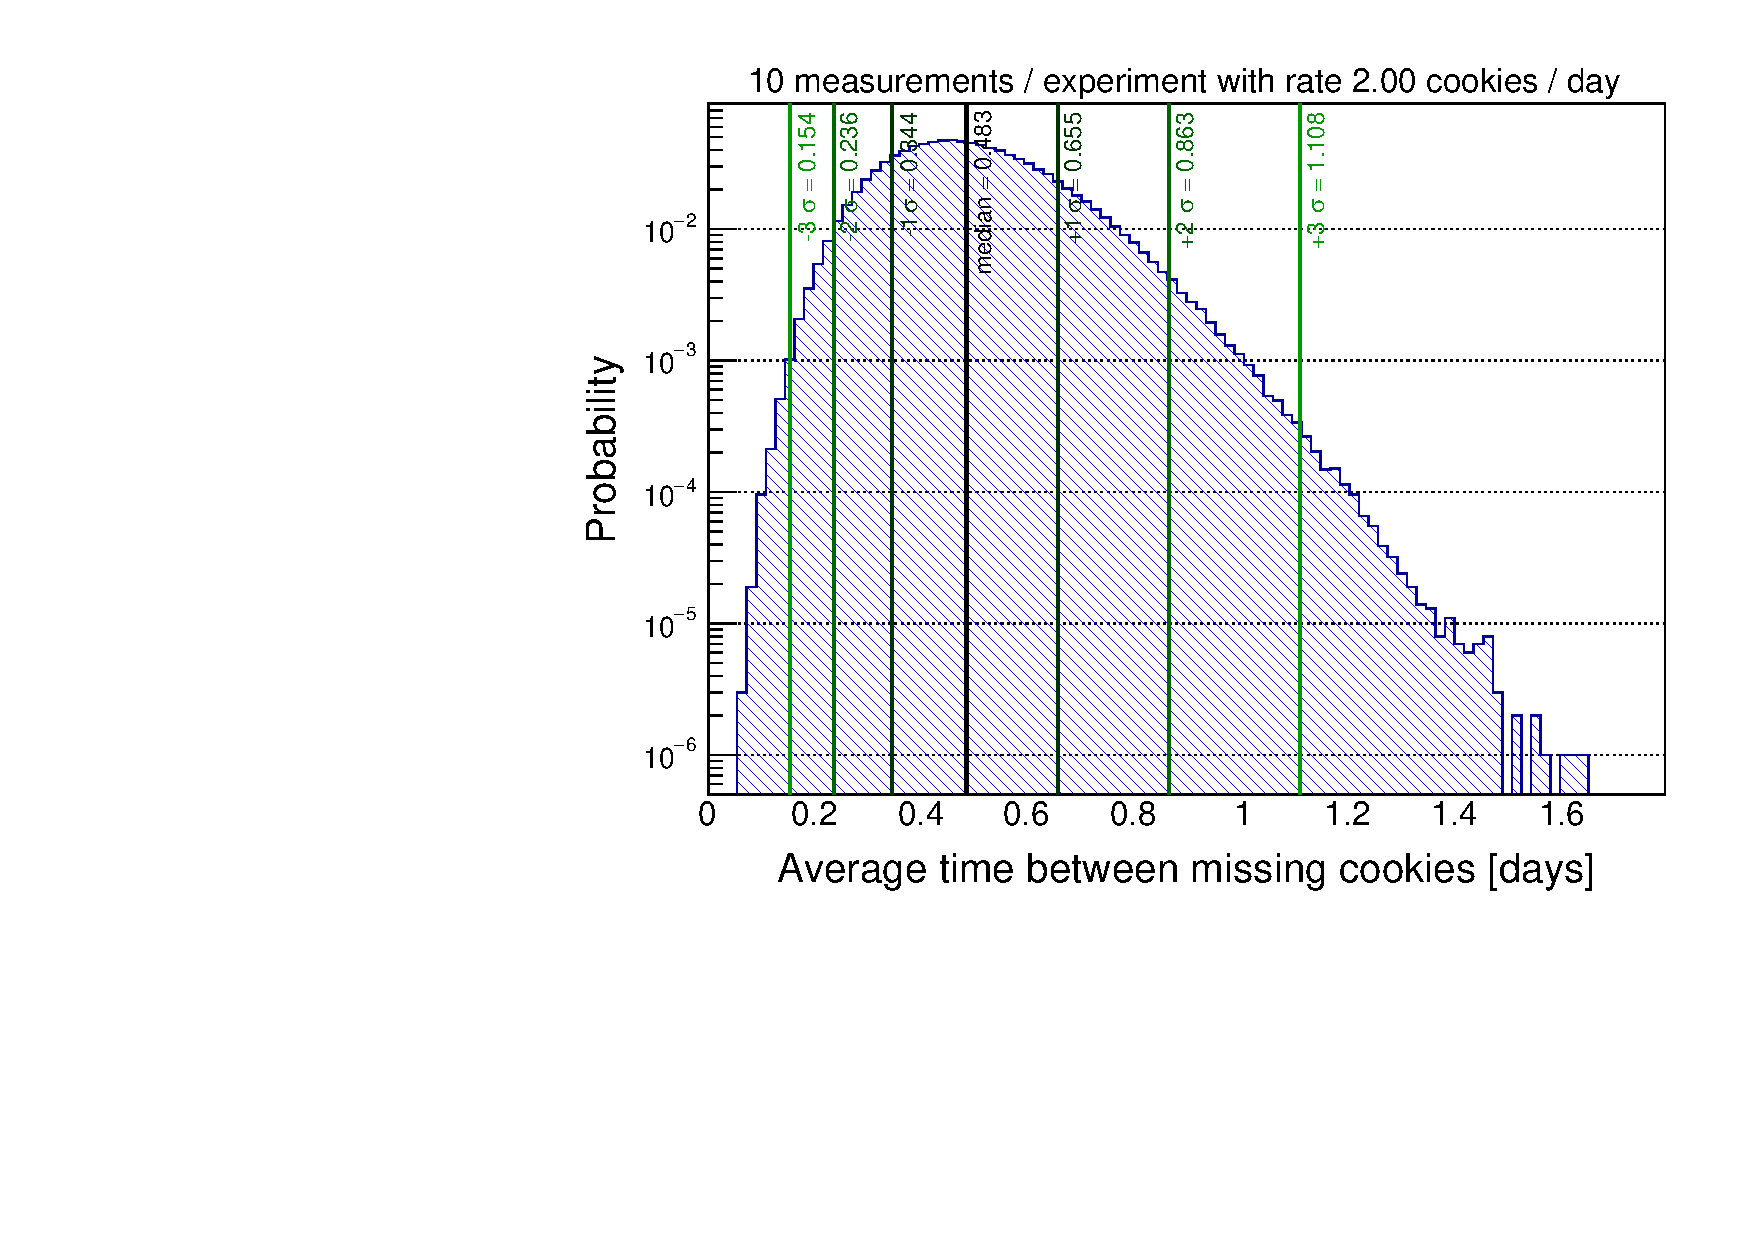
\includegraphics[width=0.49\textwidth]{fig/times_avg_dogs_quant.pdf}
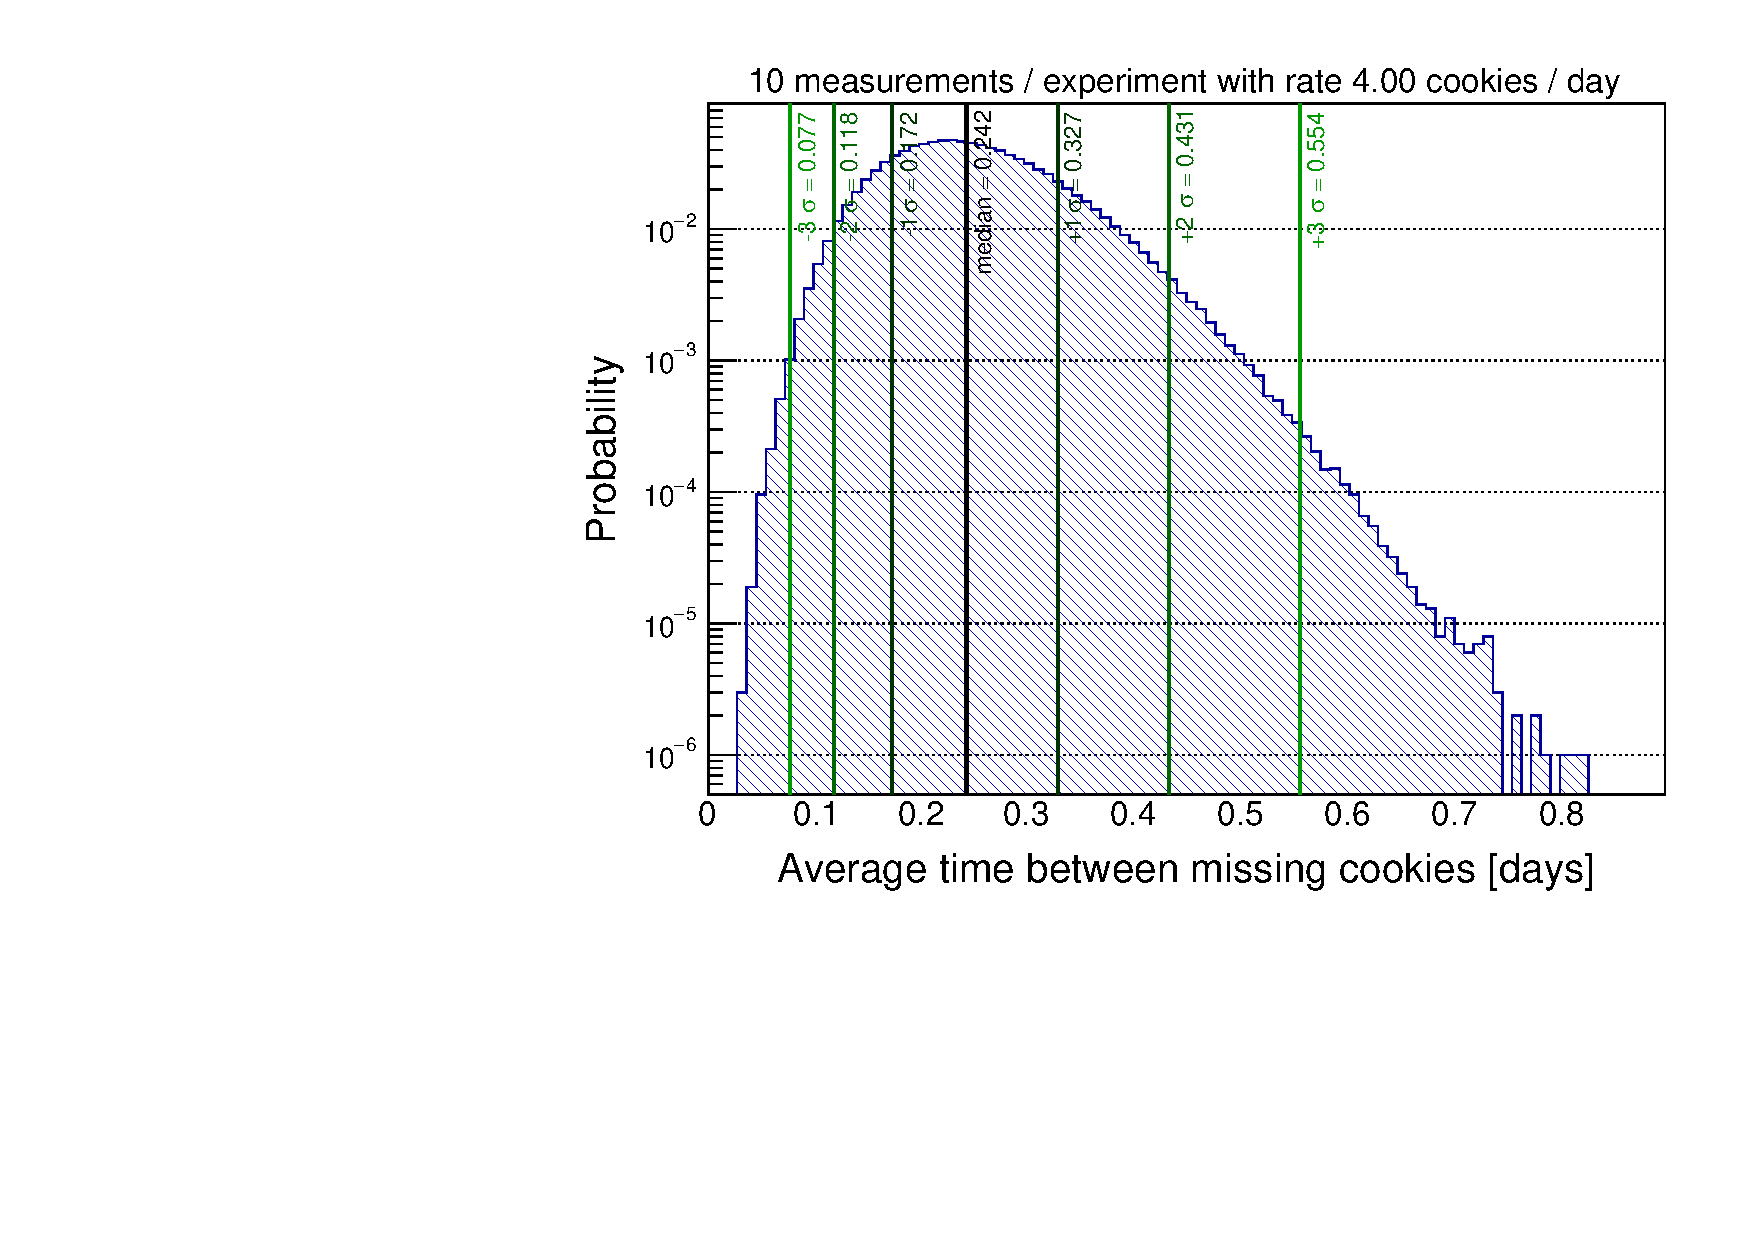
\includegraphics[width=0.49\textwidth]{fig/times_avg_aliens_quant.pdf}
\caption{{\small Simulations of the average time recorded in between missing cookies for two different hypotheses. (Left) Average time between missing cookies for dogs eating cookies (rate parameter $\lamda = 2$ cookies/day). (Right) Average time between missing cookies for aliens eating cookies (rate parameter $\lamda = 4$ cookies/day). Each entry corresponds to one simulated experiment, with 10 time measurements averaged per experiment. There are 1 million experiments simulated for each hypothesis. Shown in the figures are the median expected average time, along with the 1, 2, and 3 $\sigma$ confidence intervals (symmetric around the median)}}
\label{fig:somedata}
\end{center}  
\end{figure}

If I need to cite a reference, I can add it to my \texttt{main.bib} file and cite it like this~\cite{PhysRevD.57.3873}

\clearpage
\section{Analysis \label{sec:analysis}}

\section{Conclusion \label{sec:conclusion}}

\bibliographystyle{myutphys}
\renewcommand{\refname}{Here are the references}
\bibliography{main}

\end{document}
